%
% main.tex
%

% notes = hide | show | only
\documentclass[xcolor=dvipsnames,dvip,notes=show,table]{beamer}

% Para crear una versión 'handout' (impresa)
%\documentclass[xcolor=pst,dvips,handout,notes=show]{beamer}

%
% cabeceras.tex
%

%\usepackage[T1]{fontenc}

\definecolor{ZurichBlue}{rgb}{.255,.41,.884}

\beamertemplateshadingbackground{white!10}{white!10}

\usepackage{beamerthemeWarsaw}
\usepackage{longtable}

%\usecolortheme[named=OliveGreen]{structure} 
\setbeamertemplate{items}[ball] 
\setbeamertemplate{blocks}[rounded][shadow=true] 
\setbeamertemplate{footline}[page number]
\addtocounter{framenumber}{-1}
%Handout
%\usepackage{handoutWithNotes}
%\usepackage{tikz,times}
%\pgfpagesuselayout{2 on 1 with notes}[a4paper,border shrink=5mm]

\usepackage{beamerthemeshadow}
 \useoutertheme[hooks]{tree}
 
% \setbeamertemplate{headline}[default] % The default is just an empty headline.
% \setbeamertemplate{headline}[infolines theme]
% \setbeamertemplate{headline}[miniframes theme]
% \setbeamertemplate{headline}[sidebar theme]
% \setbeamertemplate{headline}[smoothtree theme]
% \setbeamertemplate{headline}[smoothbars theme]
% \setbeamertemplate{headline}[tree]
\beamertemplatetransparentcovereddynamic

% spanish
\usepackage[english]{babel}
\usepackage[utf8]{inputenc}

% diagramas
%\usepackage{pst-eps,epstopdf}
\usepackage{pst-node}
%\usepackage{pst-all}
\usepackage{pst-blur}
%\usepackage{pst-tree}

% incrustaciones de código fuente
\usepackage{listings}

% matemáticas y símbolos
\usepackage{amsmath}
\usepackage{amssymb}
\usepackage[right]{eurosym}
\usepackage{ulem}

% colores
\usepackage{colortbl}

%\usepackage{algorithm2e}
%\usepackage{algorithm}
%\usepackage{algorithmic}


\lstset{%
  language=Python,
	basicstyle=\footnotesize\sffamily,
	keywordstyle=\color{darkred},
 	stringstyle=\color{violet},
 	commentstyle=\color{blue},
 	showspaces=false,
 	showtabs=false,
 	showstringspaces=false,
 	frame=trBL,
        frameround=tttt,
       % backgroundcolor=\color{lightyellow},
 	extendedchars=true,
 	numbers=none,
        aboveskip=0.5cm,
        belowskip=0.5cm,
        xleftmargin=1cm,
        xrightmargin=1cm,
	breaklines=true
}
\definecolor{darkred}{rgb}{0.5, 0, 0}
\definecolor{violet}{rgb}{1, 0, 1}
\definecolor{lightyellow}{rgb}{1,1,0.8}


\usepackage{latexsym}
\usepackage{amsmath}
\usepackage{amssymb}
\usepackage{amsthm}

\usepackage{xspace}

\newcommand{\si}{$\oplus$\xspace}
\newcommand{\no}{$\ominus$\xspace}
\newcommand{\na}{$\odot$\xspace}

%Extraer
\newcommand{\linkeddata}{\textit{Linked Data}\xspace}
\newcommand{\opendata}{\textit{Open Data}\xspace}
\newcommand{\lod}{\textit{Linking Open Data}\xspace}
\newcommand{\ogd}{\textit{Open Government Data}\xspace}
\newcommand{\datasets}{\textit{datasets}\xspace}
\newcommand{\dataset}{\textit{dataset}\xspace}
\newcommand{\provenance}{\textit{provenance}\xspace}
\newcommand{\trust}{\textit{trust}\xspace}
\newcommand{\egov}{\textit{e-government}\xspace}
\newcommand{\pusi}{\textit{Public Sector Information}\xspace}
\newcommand{\gd}{\textit{Government Data}\xspace}
\newcommand{\wod}{Web de Datos\xspace}
\newcommand{\wode}{\textit{Web of Data}\xspace}
\newcommand{\eproc}{\textit{e-Procurement}\xspace}
\newcommand{\gld}{\textit{Government Linked Data}\xspace}

\hyphenation{real}

\newrgbcolor{ColorEncabezadoTabla}{0.7 0.7 0.9}
\newrgbcolor{ColorFila1}{0.8 0.8 0.7}
\newrgbcolor{ColorFila2}{0.8 0.7 0.8}
\newrgbcolor{ColorTotal}{0.7 0.9 0.7}


% \usepackage{tikz,times}
% \usetikzlibrary{mindmap,backgrounds}




%%%%%%%%%%%%%%%%%%%%%%%%%%%%%%%%%%%%%%%%%%%%%%%%%%%%%%%%%%%%%%%%%%%%%%

\title[MapReduce Intro]{The MapReduce Programming Model}
\author[Dr. Jose Mar\'{i}a Alvarez-Rodr\'{i}guez]{\textbf{Introduction and Examples}\\ \vspace{0.3cm} Dr. Jose Mar\'{i}a Alvarez-Rodr\'{i}guez \\ \vspace{0.3cm} ``Quality Management in Service-based Systems and Cloud Applications'' \\ \vspace{0.3cm} FP7 RELATE-ITN}
\subtitle{}
\institute{South East European Research Center}


\date{Thessaloniki, 20th of April, 2013}

\begin{document}

\frame{
\titlepage

}

\frame{
\tableofcontents

}


%%%%%%%%%%%%%%%%%%%%%%%%%%%%%%%%%%%%%%%%%%%%%%%%%%%%%%%%%%%%%%%%%%%%%%
\section{MapReduce in a nutshell}


\frame{
  \frametitle{Features}

\begin{block}{A programming model...}
\begin{enumerate}
 \item Large-scale distributed data processing
 \item Simple but restricted
 \item Paralell programming
 \item Extensible
\end{enumerate}
\end{block}

}


\begin{frame}[fragile]
  \frametitle{Antecedents}

\begin{alertblock}{Functional programming}<1->
\begin{enumerate}
 \item Inspired
 \item ...but not equivalent
\end{enumerate}
\end{alertblock}

\begin{exampleblock}{Example in Python}<2->
``Given a list of numbers between 1 and 50 print only even numbers''
\begin{lstlisting}
print filter(lambda x: x % 2 == 0, range(1, 50))
\end{lstlisting}
\tiny
\begin{itemize}
 \item A list of numbers (data)
 \item A condition (even numbers)
 \item A function \textit{filter} that is applied to the list (map)
\end{itemize}
\end{exampleblock}



\end{frame}


\begin{frame}[fragile]
  \frametitle{...Other examples...}

\begin{exampleblock}{Example in Python}
``Return the sum of the squares of a list of numbers between 1 and 50''
\begin{lstlisting}
import operator
reduce(operator.add, map((lambda x: x **2), range(1,50)) , 0)
\end{lstlisting}

\end{exampleblock}


\begin{itemize}
 \item ``reduce'' is equivalent to ``foldl'' in other func. languages as Haskell
 \item other math considerations should be taken into account (kind of operator)...
\end{itemize}

\end{frame}


\frame{
  \frametitle{Some interesting points...}

\begin{alertblock}{The Map Reduce framework...}
\begin{enumerate}
 \item Inspired in functional programming concepts (\textbf{but not equivalent})
 \item Problems that can be paralellized
 \item Sometimes recursive solutions
 \item ...
\end{enumerate}
\end{alertblock}

}

\frame{
  \frametitle{Basic Model}
\begin{figure}[!htb]
\centering
 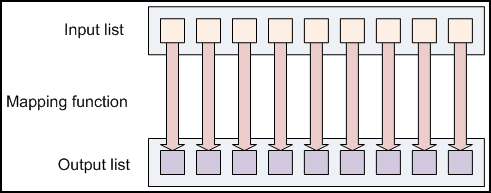
\includegraphics[width=7cm]{img/mapping-hadoop}
 \end{figure}

\tiny
``MapReduce: The Programming Model and Practice'', SIGMETRICS, Turorials 2009, Google.

}



\frame{
  \frametitle{Map Function}
\begin{figure}[!htb]
\centering
 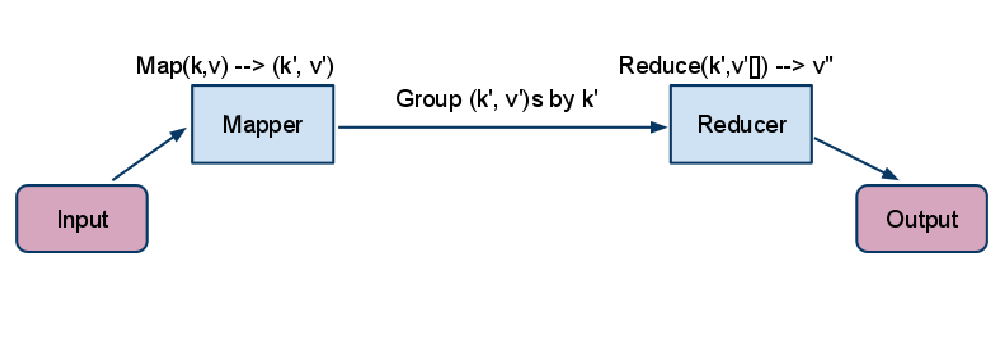
\includegraphics[width=7cm]{img/basic-model-mapreduce}
 \caption{Mapping creates a new output list by applying a function to individual elements of an input list.}
\end{figure}

\tiny
``Module 4: MapReduce'', Hadoop Tutorial, Yahoo!.
}

\frame{
  \frametitle{Reduce Function}
\begin{figure}[!htb]
\centering
 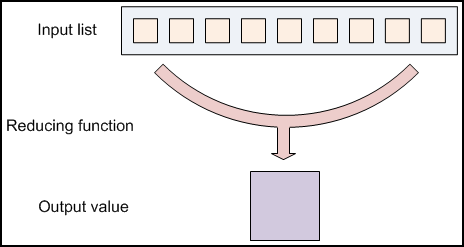
\includegraphics[width=7cm]{img/reduce}
 \caption{Reducing a list iterates over the input values to produce an aggregate value as output.}
\end{figure}

\tiny
``Module 4: MapReduce'', Hadoop Tutorial, Yahoo!.
}



\frame{
  \frametitle{MapReduce Flow}
\begin{figure}[!htb]
\centering
 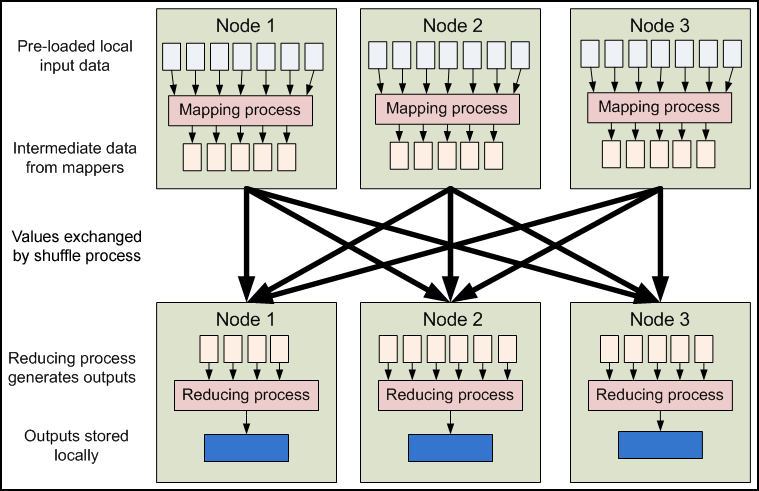
\includegraphics[width=7cm]{img/flow}
 \caption{High-level MapReduce pipeline.}
\end{figure}

\tiny
``Module 4: MapReduce'', Hadoop Tutorial, Yahoo!.
}

\frame{
  \frametitle{MapReduce Flow}
\begin{figure}[!htb]
\centering
 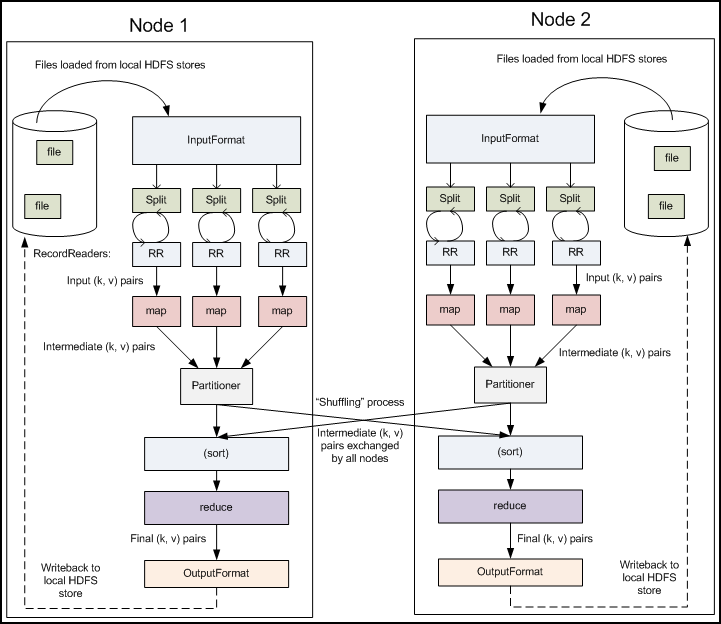
\includegraphics[width=7cm]{img/high-level}
 \caption{Detailed Hadoop MapReduce data flow.}
\end{figure}

\tiny
``Module 4: MapReduce'', Hadoop Tutorial, Yahoo!.
}




\frame{
  \frametitle{Tip}
\begin{exampleblock}{What is MapReduce?}
It is a \textbf{framework} inspired in \textbf{functional programming} to tackle problems in which steps 
can be \textbf{paralellized} applying a \textbf{divide and conquer} approach.
\end{exampleblock}

}

\section{Thinking in MapReduce}

\frame{
  \frametitle{When should I use MapReduce?}
  \scriptsize
\begin{exampleblock}{Query}<1->
\begin{itemize}
 \item Index and Search: inverted index
 \item Filtering
 \item Classification 
 \item Recommendations: clustering or collaborative filtering
\end{itemize}
\end{exampleblock}

\begin{block}{Analytics}<2->
\begin{itemize}
 \item Summarization and statistics
 \item Sorting and merging 
 \item Frequency distribution
 \item SQL-based queries: group-by, having, etc.
 \item Generation of graphics: histograms, scatter plots.
\end{itemize}

\end{block}

\begin{alertblock}{Others}<3->
 Message passing such as Breadth First-Search or PageRank algorithms.
\end{alertblock}


}


\frame{
  \frametitle{How Google uses MapReduce (80\% of data processing)...}

\begin{itemize}
\item Large-scale web search indexing
\item Clustering problems for Google News
\item Produce reports for popular queries, e.g. Google Trend
\item Processing of satellite imagery data
\item Language model processing for statistical machine translation
\item Large-scale machine learning problems
\item \ldots
\end{itemize}


}

\frame{
  \frametitle{Comparison of MapReduce and other approaches}
\begin{figure}[!htb]
\centering
 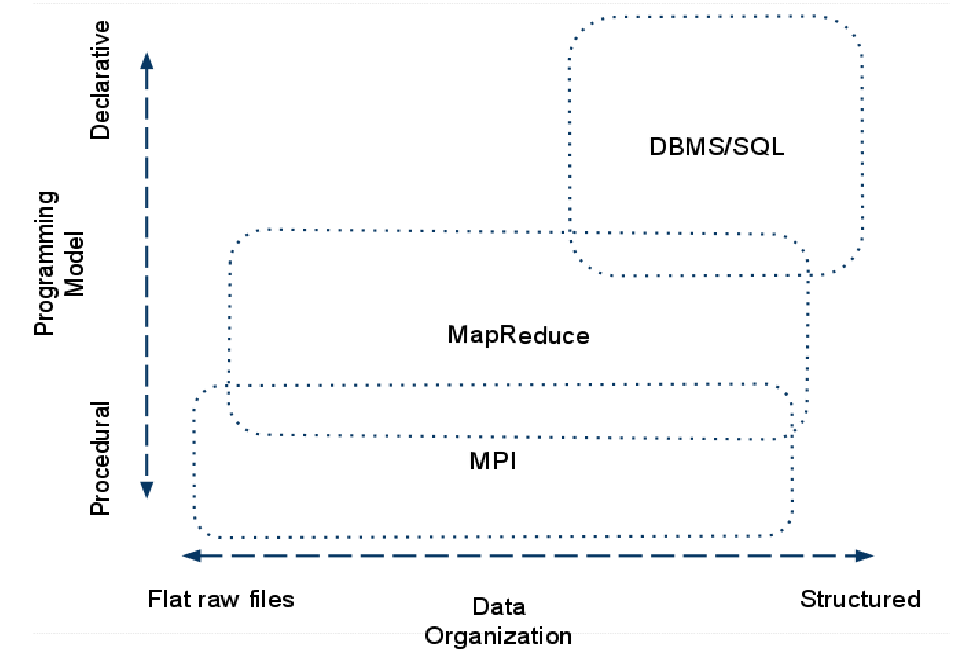
\includegraphics[width=8cm]{img/comparison-map-reduce}
\end{figure}

\tiny
``MapReduce: The Programming Model and Practice'', SIGMETRICS, Turorials 2009, Google.

}

\frame{
  \frametitle{Evaluation of MapReduce and other approaches}
\begin{figure}[!htb]
\centering
 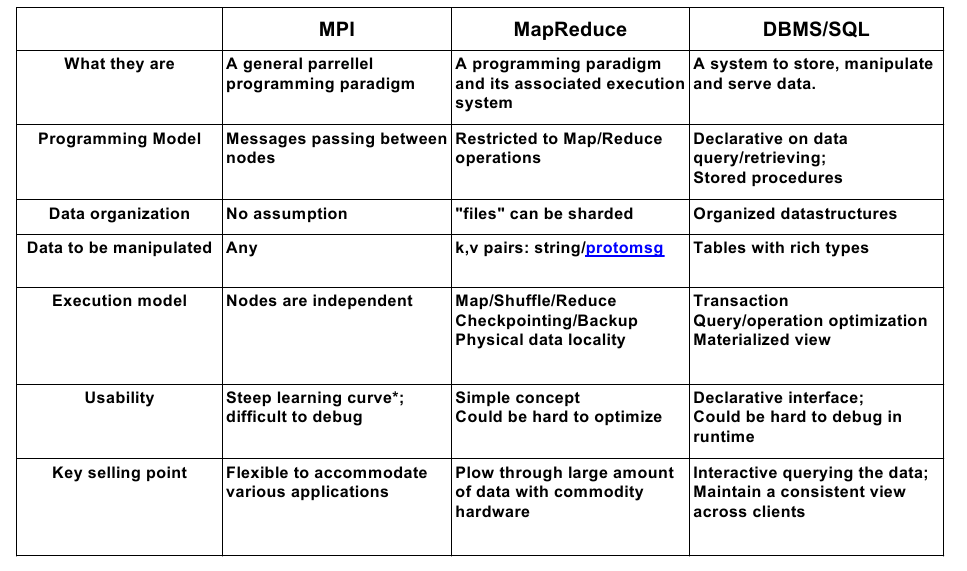
\includegraphics[width=8cm]{img/table-features}
\end{figure}

\tiny
``MapReduce: The Programming Model and Practice'', SIGMETRICS, Turorials 2009, Google.

}


\frame{
  \frametitle{Apache Hadoop}

\begin{columns}[c] % the "c" option specifies center vertical alignment
\column{.5\textwidth} % column designated by a command


\begin{block}{MapReduce definition}
The Apache Hadoop software library is a \textbf{framework} that allows for the \textbf{distributed processing} of \textbf{large data sets} across \textbf{clusters} of computers using \textbf{simple programming model}s.
\end{block}


\column{.5\textwidth}

\begin{figure}[htb]
\centering
	
\includegraphics[width=3cm]{img/hadoop-logo}
\caption{Apache Hadoop Logo.}
\end{figure}

\end{columns}

}


\frame{
  \frametitle{Tip}
\begin{exampleblock}{What can I do in MapReduce?}
Three main functions:
\begin{enumerate}
 \item \textbf{Querying}
 \item \textbf{Summarizing}
 \item \textbf{Analyzing}
\end{enumerate}
\ldots \textbf{large datasets} in \textbf{off-line} mode for \textbf{boosting} other \textbf{on-line} processes.
\end{exampleblock}

}

\section{Applying MapReduce}

\frame{
  \frametitle{MapReduce in Action}
\begin{block}{MapReduce Patterns}
\begin{enumerate}
 \item Summarization
 \item Filtering
 \item Data Organization
 \item SQL-based (Join)
 \item Others: metapatterns, input-output, etc. (depending on the implementation)
\end{enumerate}
\end{block}

}


\frame{
  \frametitle{Summarization}
\begin{exampleblock}{Types}
\begin{enumerate}
 \item Numerical summarizations
 \item Inverted index
 \item Counting and counters
 \end{enumerate}
\end{exampleblock}

}


\frame{
  \frametitle{Numerical Summarization-I}
\begin{block}{Description}
A general pattern for calculating aggregate statistical values over your data.
\end{block}

\begin{alertblock}{Intent}
Group records together by a key field and calculate a numerical aggregate per group to
get a top-level view of the larger data set.
\end{alertblock}

}

\frame{
  \frametitle{Numerical Summarization-II}
  
\begin{block}{Applicability}
\begin{itemize}
 \item To deal with numerical data or counting.
 \item To group data by specific fields
\end{itemize}
\end{block}

\tiny
\begin{exampleblock}{Examples}
\begin{enumerate}
 \item Word count
 \item Record count
 \item Min/Max/Count
 \item Average/Median/Standard deviation
 \item \ldots
\end{enumerate}

\end{exampleblock}

}


\begin{frame}[fragile]
  \frametitle{Numerical Summarization-Pseudocode}
\begin{verbatim}
 class Mapper
   method Map(recordid id, record r)
      for all term t in record r do
         Emit(term t, count 1)
 
class Reducer
   method Reduce(term t, counts [c1, c2,...])
      sum = 0
      for all count c in [c1, c2,...] do
          sum = sum + c
      Emit(term t, count sum)      
\end{verbatim}
\end{frame}    

\begin{frame}[fragile]
  \frametitle{Numerical Summarization-Word Counter}

\begin{lstlisting}[language=Java]
public void map(LongWritable key, Text value, Context context) 
      throws Exception {
        String line = value.toString();
        StringTokenizer tokenizer = new StringTokenizer(line);
        while (tokenizer.hasMoreTokens()) {
            word.set(tokenizer.nextToken());
            context.write(word, one);
        }
    }
    
public void reduce(Text key, Iterable<IntWritable> values, Context context) 
      throws IOException, InterruptedException {
        int sum = 0;
        for (IntWritable val : values) {
            sum += val.get();
        }
        context.write(key, new IntWritable(sum));
    }    
\end{lstlisting}

\end{frame}


\frame{
  \frametitle{Example-II}

\begin{block}{Min/Max}
 Given a list of tweets (username, date, text) determine first and last time an user commented and the number of times.
\end{block}

\tiny
\begin{exampleblock}{Implementation}
 See \url{https://github.com/chemaar/seqos/tree/master/prototypes/mapreduce-intro}
\end{exampleblock}

}


\begin{frame}[fragile]
  \frametitle{Example II-Min/Max, function Map}

\begin{lstlisting}[language=Java]
public void map(Object key, Text value, Context context)
      throws IOException, InterruptedException, ParseException {
        Map<String, String> parsed = MRDPUtils.parse(value.toString());
        String strDate = parsed.get(MRDPUtils.CREATION_DATE);
        String userId = parsed.get(MRDPUtils.USER_ID);
        if (strDate == null || userId == null) {
          return;
        }
        Date creationDate = MRDPUtils.frmt.parse(strDate);
        outTuple.setMin(creationDate);
        outTuple.setMax(creationDate);
        outTuple.setCount(1);
        outUserId.set(userId);
        context.write(outUserId, outTuple);
}
\end{lstlisting}

\end{frame}

\begin{frame}[fragile]
  \frametitle{Example II-Min/Max, function Reduce}

\begin{lstlisting}[language=Java]
public void reduce(Text key, Iterable<MinMaxCountTuple> values,
      Context context) throws IOException, InterruptedException {
      result.setMin(null);
      result.setMax(null);
      int sum = 0;
      for (MinMaxCountTuple val : values) {
            if (result.getMin() == null
                  || val.getMin().compareTo(result.getMin()) < 0) {
                  result.setMin(val.getMin());
            }
            if (result.getMax() == null
                  || val.getMax().compareTo(result.getMax()) > 0) {
                  result.setMax(val.getMax());
                  }
                  sum += val.getCount();}
      result.setCount(sum);
      context.write(key, result);
}
\end{lstlisting}

\end{frame}


\frame{
  \frametitle{Example-III}

\begin{block}{Average}
Given a list of tweets (username, date, text) determine the average comment length per hour of day.
\end{block}

\tiny
\begin{exampleblock}{Implementation}
 See \url{https://github.com/chemaar/seqos/tree/master/prototypes/mapreduce-intro}
\end{exampleblock}

}


\begin{frame}[fragile]
  \frametitle{Example III-Average, function Map}

\begin{lstlisting}[language=Java]
public void map(Object key, Text value, Context context)
      throws IOException, InterruptedException,ParseException {
      Map<String, String> parsed = 
            MRDPUtils.parse(value.toString());
      String strDate = parsed.get(MRDPUtils.CREATION_DATE);
      String text = parsed.get(MRDPUtils.TEXT);
      if (strDate == null || text == null) {
            return;
      }
      Date creationDate = MRDPUtils.frmt.parse(strDate);
      outHour.set(creationDate.getHours());
      outCountAverage.setCount(1);
      outCountAverage.setAverage(text.length());
      context.write(outHour, outCountAverage);
}
\end{lstlisting}

\end{frame}

\begin{frame}[fragile]
  \frametitle{Example III-Average, function Reduce}

\begin{lstlisting}[language=Java]
public void reduce(IntWritable key, Iterable<CountAverageTuple> values,
      Context context) throws IOException, InterruptedException {
      float sum = 0;
      float count = 0;
      for (CountAverageTuple val : values) {
            sum += val.getCount() * val.getAverage();
            count += val.getCount();
      }
      result.setCount(count);
      result.setAverage(sum / count);
      context.write(key, result);
}
\end{lstlisting}

\end{frame}



\begin{frame}[fragile]
  \frametitle{Numerical Summarization-III}
  \begin{block}{Relation to SQL}<1->
  
  \begin{lstlisting}
SELECT MIN(numcol1), MAX(numcol1),
COUNT(*) FROM table GROUP BY groupcol2;
\end{lstlisting}
\end{block}

\begin{exampleblock}{Implementation in PIG}<2->

\begin{lstlisting}
b = GROUP a BY groupcol2;
c = FOREACH b GENERATE group, MIN(a.numcol1),
MAX(a.numcol1), COUNT_STAR(a);
\end{lstlisting}

\end{exampleblock}

\end{frame}


\frame{
  \frametitle{Filtering}
\begin{exampleblock}{Types}
\begin{enumerate}
 \item Filtering
 \item Top N records
 \item Bloom filtering 
 \item Distinct
 \end{enumerate}
\end{exampleblock}

}





\frame{
  \frametitle{Filtering-I}
\begin{block}{Description}
It evaluates each record separately and decides, based on some condition, whether it should stay or go.
\end{block}

\begin{alertblock}{Intent}
Filter out records that are not of interest and keep ones that are.
\end{alertblock}

}
\frame{
  \frametitle{Filtering-II}
  
\begin{block}{Applicability}
To collate data
\end{block}

\tiny
\begin{exampleblock}{Examples}
\begin{enumerate}
 \item Closer view of dataset
 \item Data cleansing
 \item Tracking a thread of events
 \item Simple random sampling
 \item Distributed Grep
 \item Removing low scoring dataset
 \item Log Analysis
 \item Data Querying
 \item Data Validation
 \item \ldots
\end{enumerate}
\end{exampleblock}

}


\begin{frame}[fragile]
  \frametitle{Filtering-Pseudocode}
\begin{verbatim}
class Mapper
   method Map(recordid id, record r)
      field f = extract(r)
      if predicate (f)       
         Emit(recordid id, value(r))
 
class Reducer
   method Reduce(recordid id, values [r1, r2,...])
      //Whatever      
      Emit(recordid id, aggregate (values))      
\end{verbatim}
\end{frame}    



\frame{
  \frametitle{Example-IV}

\begin{block}{Distributed Grep}
Given a list of tweets (username, date, text) determine the tweets that contain a \textit{word}.
\end{block}

\tiny
\begin{exampleblock}{Implementation}
 See \url{https://github.com/chemaar/seqos/tree/master/prototypes/mapreduce-intro}
\end{exampleblock}

}


\begin{frame}[fragile]
  \frametitle{Example IV-Distributed Grep, function Map}

\begin{lstlisting}[language=Java]
public void map(Object key, Text value, Context context)
      throws IOException, InterruptedException {
      Map<String, String> parsed = 
            MRDPUtils.parse(value.toString());
      String txt = parsed.get(MRDPUtils.TEXT);
      String mapRegex = ".*\\b"+context.getConfiguration()
            .get("mapregex")+"(.)*\\b.*";
      if (txt.matches(mapRegex)) {
            context.write(NullWritable.get(), value);
      }
}
\end{lstlisting}
\tiny

\begin{alertblock}{...and the Reduce function?}
 In this case it is not necessary and output values are directly writing to the output.
\end{alertblock}

\end{frame}


\begin{frame}[fragile]
  \frametitle{Filtering-III}
  \begin{block}{Relation to SQL}<1->
  
  \begin{lstlisting}
SELECT * FROM table WHERE colvalue < 3;
\end{lstlisting}
\end{block}

\begin{exampleblock}{Implementation in PIG}<2->

\begin{lstlisting}
b = FILTER a BY colvalue < 3;
\end{lstlisting}

\end{exampleblock}

\end{frame}




\frame{
  \frametitle{Tip}
\begin{exampleblock}{How can I use MapReduce ?}

\end{exampleblock}

}


\frame{
  \frametitle{Tip}
\begin{exampleblock}{How can I run a MapReduce framework?}

\end{exampleblock}

}

\section{Success Stories with MapReduce}


\frame{
  \frametitle{Tip}
\begin{exampleblock}{Who is using MapReduce?}

\end{exampleblock}

}

\section{Beyond MapReduce}


\frame{
  \frametitle{Tip}
\begin{exampleblock}{What's next?}

\end{exampleblock}

}




\section{Summary and Conclusions}

\frame{
\titlepage

}



\section{Future Work}

\frame{
\titlepage

}



\nocite{*}
% \section*{Acknowledgements}
% \frame{
%   \frametitle{All have contributed...} 
% \begin{figure}[!htb]
% \centering
%  \includegraphics[width=9cm]{imgs/linkedin}
% \end{figure}
% }

%%%%%%%%%%%%%%%%%%%%%%%%%%%%%%%%%%%%%%%%%%%%%%%%%%%%%%%%%%%%%%%%%%%%%%
\appendix
\section*{References}
\bibliographystyle{abbrv}
\bibliography{references}
% 
% 
%\section*{Preguntas}
% \input{preguntas-preparadas}


\end{document}

